\large\zihao{-4}
%---------------------------------------
\section{关于模板的一些说明}%\label{chpt:1}
%---------------------------------------
本模版\glossary{模板}是为{\university\school}本科毕业生撰写毕业论文而设计的,版面尺寸按照{\school}的论文撰写要求选取。模板的第一版是
2006年完成的,经过多年的使用、 改进,最终发展成目前的版本。

第一次使用本模版时,请先阅读~\ref{subsec:1}节;如果安装\CTeX{}\index{\CTeX}有问题,请阅读~\ref{sec:versionSelect}节;如果对数学公式、符号或定义、定理、证明等各种命令环境不熟悉,请阅读第~\ref{sec:2two}
节;如果对表格或图形的\index{图形插入}插入不熟悉,请阅读第~\ref{sec:ssss}节;如果对\index{交叉引用}交叉引用\index{交叉引用}不熟悉,请阅读第~\ref{sec_si4}节。 如果想了解在~\LaTeX 中\index{程序引入}引入程序代码,如
~{\tt Matlab},{\tt Mathematica},{\tt R} 和~{\tt C/C++} 等的代码,请阅读第~\ref{sec:codeinludsion}节并分别参考附录~\ref{appendix:A}、~\ref{appendix:B}、~\ref{appendix:C}、\ref{appendix:D} 中的实例。
\subsection{模板的构成}\label{subsec:1}
本模板由若干文件组成,所有文件都存放在一个主文件夹\index{文件夹}里。为了使用和管理方便,在主文件夹中又分了五个子文件夹:{\tt codes, biaoge, filesforteachers, preample, tables},其中~{\tt preample\index{文件夹!preample}, tables\index{文件夹!table}} 中的文件一般不用管,
而~{\tt codes\index{文件夹!codes}} 在熟悉模板后可以删除。文件夹~{\tt biaoge\index{文件夹!biaoge}} 包含一些由学生填写的表格文件,而文件夹~{\tt filesforteachers\index{文件夹!filesforteachers}} 则包含一些由教师填写的表格文件(当然也可由学生复制进去)。模板由主文件~{\tt mytemplate.tex\index{mytemplate.tex}} 及五类子文件构成:
\begin{enumerate}
  \item 论文的编译通过主文件才能进行。学生的基本信息,如姓名,学号,论文题目等,都在主文件上输入。
  \item\label{item:2} 这一类文件是论文的主要组成部分,由学生完成。有以下几个文件:
  \begin{enumerate}
    \item {\tt abstract.tex\index{abstract.tex}},这是论文的摘要。
    \item {\tt body.tex\index{body.tex}},这是论文的正文部分。
    \item {\tt bibfile.tex\index{bibfile.tex}},这是论文的参考文献。
    \item {\tt thanks.tex\index{thanks.tex}},这是论文的致谢词部分。
  \end{enumerate}
  以上两类文件都存放在主文件夹里,学生只须在相关的文件中按~\LaTeX\index{\LaTeX} 的要求及文件中的提示输入相应的内容即可。
  %\item 这一类是三个与教师有关的文件:
  %\begin{enumerate}
  %  \item\label{term1} {\tt zhidaojiaoshigeifen.sty},这个文件包含指导教师评分及评阅意见,由指导教师完成。
  %  \item {\tt jiaochageifen.sty},这个文件包含交叉评阅意见及评分,由负责交叉评阅的教师完成。
  %  \item {\tt dabianchengji.sty},这个文件包含答辩评审意见、答辩分数及论文成绩,由教师答辩小组组长完成。
  %\end{enumerate}
  %这类文件存放在子文件夹~{\tt filesforteachers} 中。相关教师只须在对应的文件中按\LaTeX
  %的要求及文件中的提示输入相应的内容即可。具体的对应文件及填写方法参看后面表格(开题报告二~\pageref{table:kaiti_2},教师评阅表~\pageref{table:pingyue},交叉评阅表%~\pageref{table:jiaochapingyue},答辩记录表~\pageref{table:dabianjilu})中的说明。
  \item 这一类有四个文件:
  \begin{enumerate}
    \item {\tt kaiti\_1.tex\index{kaiti\_1.tex}}(开题报告一);
    \item {\tt kaiti\_2.tex\index{kaiti\_2.tex}}(开题报告二);
    %\item {\tt renwu.tex}(任务书);
    \item {\tt dabianjilu.tex\index{dabianjilu.tex}}(答辩记录)。
  \end{enumerate}
   这类文件存放在子文件夹~{\tt biaoge} 中。前两个文件是开题报告,最后一个文件是答辩记录。完成人只须在对应的文件中按~\LaTeX 的要求及文件中的提示输入相应的内容即可。
   具体的对应文件及填写方法参看后面表格(第~\pageref{table:kaiti_1} 页开题报告一,第~\pageref{table:kaiti_2} 页开题报告二,第~\pageref{table:dabianjilu} 页答辩记录表)中的说明。
  \item\label{item:4} 这一类是三个与教师有关的文件:
  \begin{enumerate}
    \item\label{term1} {\tt zhidaojiaoshigeifen.tex\index{zhidaojiaoshigeifen.tex}},这个文件包含指导教师评分及评阅意见,由指导教师完成。
    \item {\tt jiaochageifen.tex\index{jiaochageifen.tex}},这个文件包含交叉评阅意见及评分,由负责交叉评阅的教师完成。
    \item {\tt dabianchengji.tex\index{dabianchengji.tex}},这个文件包含答辩评审意见及论文评定成绩,由教师答辩小组组长完成。
  \end{enumerate}
  这类文件存放在子文件夹~{\tt filesforteachers} 中。相关教师只须在对应的文件中按~\LaTeX
  的要求及文件中的提示输入相应的内容即可。具体的对应文件及填写方法参看后面表格(第~\pageref{table:kaiti_2} 页开题报告二,第~\pageref{table:pingyue} 页指导教师评阅表,第~\pageref{table:jiaochapingyue} 页交叉评阅表
  ,第~\pageref{table:dabianjilu} 页答辩记录表)中的说明。
  \item\label{item:head} 这一类中除头文件{ \tt SWUthesis.sty\index{SWUthesis.sty}} 外还有一些诸如学校的~logo 和学院的~logo 之类的文件。
        这几个文件单独放在子文件夹~{\tt preample} 中,这些文件一般不用改动。

      %这四类文件在前面相关的内容录入后,通过编译主文件,会自动将指导教师评阅意见,交叉评阅意见以及答辩记录,答辩分数和论文等级等相关的内容导入对应表格,最后生成~PDF 格式的文件。
  \item\label{item:miscellanceous} 这一类中有四个文件:{\tt coverpage.tex\index{coverpage.tex}}(封面),{\tt pingyue\_1.tex\index{pingyue\_1.tex}}(指导教师评阅表), {\tt pingyue\_2.tex\index{pingyue\_2.tex}} (交叉评阅表),
        {\tt dabian.tex}(答辩记录表)。这几个文件,单独放在子文件夹~{\tt tables} 中,它们只生成封面或表格的框架,其中需要填入的内容通过编译会自动从其它相关文件中导入,
        所以一般不用对这些文件做改动。
\end{enumerate}
总之第~\ref{item:head} 类和第~\ref{item:miscellanceous} 类的文件一般不用去管,主文件和~\ref{item:2}--~\ref{item:4} 类中的子文件在完成后由学生统一通过主文件编译,
最后生成包含所有内容和所有表格的、完整的论文的~PDF 格式的文件。子文件夹~{\tt codes} 中放有一些制作本说明时所用的一些文件,如果不需要可以删除。
\subsubsection{三级标题}
本节为测试三级标题在目录中的显示而设。
\subsection{\CTeX{} 简介}
\TeX{} 是计算机科学家、图灵奖得主~Knuth\index{Knuth} 教授设计的一款权威的科技论文排版软件!学习~\TeX(\LaTeX),
Knuth 的专著~\cite{knuth} 无疑是权威之选。该书排版堪称完美,从中可以看出大师的魅力。更重要的是~Knuth 教授无偿公开了~\TeX{} 的所有源代码,
也就是说它是开源 (Open Source)的(通俗地说就是可以免费使用)。正因为这个原因,后人在其基础上开发了~\LaTeX 。\LaTeX{} 方便好用,被广泛传播,成了当今世界科技界最权威的论文排版软件。
作为一个非常全面的~\LaTeX{} 的参考书,\cite{companion} 是一个不错的选择。如果阅读英文有困难,作为一个初学者,也可以先看看~\cite{zhanglibo}。

\TeX{} 和~\LaTeX{} 排版软件和~MS 的~Word 软件不同,后者是``所见即所得\index{所见即所得}"(WYSIWYG\index{WYSIWYG},what you see is what you get),而前者是``所想即所得\index{所想即所得}"(WYWIWYG\index{WYWIWYG},what you want is what you get)。
二者在风格上迥然不同,因此学习~\LaTeX{} 需要稍微改变一下自己的习惯。

%\paragraph{Run-in headings.}
目前国内使用的~\LaTeX{} 汉化版\index{\LaTeX{} 汉化版}称为~
\CTeX ,最新的版本为~2.9.2.164,可在~\href{http://www.ctex.org/HomePage}{\CTeX{} 网站}~\index{\CTeX 网站}免费下载安装。
\subsection{\CTeX{} 的安装\index{\CTeX 的安装}}\label{sec:versionSelect}
根据我个人及我指导过的 \nianxian 届学生的使用经历,2.4.5-8 版的\CTeX (安装文件是\\{\tt
CTeX-2.4.5-8-Full.exe})在~XP 操作系统下的问题较少,占用空间也较小,因此在~XP 操作系统下我推荐使用这个版本的~\CTeX。但在安装时要先把安装计算机上的时间调到较早的一个时间,
如$2004$年,待安装完毕运行一次后再将时间调回当前时间,否则运行时会报错。在~Win 7 或以上的操作系统下,安装~2.4.5-8 版的~\CTeX{} 可能会出现问题;而安装最新版的~
2.9.2.164(安装文件为~
CTeX~\_2.9.2.164\_Full.exe)时,DVI 阅读器~{\tt YAP}\index{YAP} 可能会报错。只需按提示点击弹出窗口相应的按钮继续安装。安装好后,如果用{ \tt LATEX} 编译,打开~DVI 文件时可能会频繁弹出
恼人的{ \tt MiKTeX Problem Report} 错误报告窗口。这个问题发生的原因我目前在网上还没有看到合理的解释,当然也没有发现有人给出过解决方法。估计发生的原因可能和操作系统有关。
通过反复琢磨和测试,我找到一个解决办法,就是在~DVI 窗口
进入{ \tt View --> Options...},这时会弹出{ \tt Options} 窗口,点击{ \tt Display},在{ \tt Default render} 右端下拉菜单中有两个选项(见图~\ref{fig:optionWin}):{\tt Pk} 和{ \tt Dvips},
选择{ \tt Dvips}作为默认值后问题即可解决。其它版本的~\CTeX{} 若出现类似地问题也可这样来解决。我在~\CTeX\_2.9.0.152 版上测试过,
用这个方法解决了同样的问题。
\begin{figure}
\centering
  % Requires \usepackage{graphicx}
  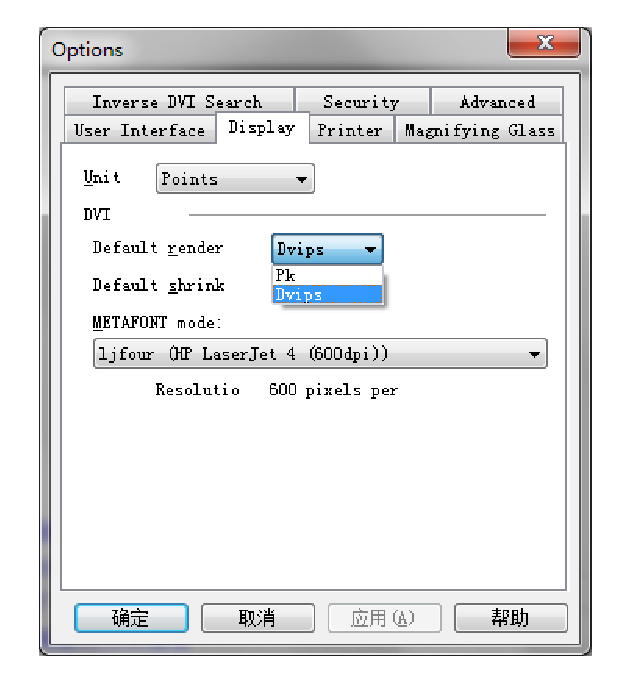
\includegraphics[width=8cm]{codes/292164wenti}\\
  \caption{{\tt Options} 窗口}\label{fig:optionWin}
\end{figure}
%---------------------------------------
\subsection{\CTeX{} 文件的编译\index{\CTeX 文件的编译}}
%---------------------------------------
在新版~\CTeX$2.9.2.164$ 下,一般情况下用{ \tt PDFLateX} 编译,直接生成PDF文件。也可用{ \tt LATEX} 编译,但速度可能会非常慢,有时甚至可能会出错。

如果用{ \tt PDFLateX} 编译后生成的PDF没有自动打开,那么就在{ \tt WinEdt} 编辑窗口的顶端点击{ \tt Options},在下拉菜单中选择{ \tt Execution Modes...},再在弹出的窗口中的第一栏中选择{ \tt PDFLaTex},在第二栏中勾选{ \tt Start Viewer}(如图~\ref{fig:optionPDF}),然后点击{ \tt OK}收起窗口,之后再编译即可。
\begin{figure}
  \centering
  % Requires \usepackage{graphicx}
  \includegraphics[width=16cm]{options.png}\\
  \caption{编译后自动打开PDF文件的设置}\label{fig:optionPDF}
\end{figure}

%---------------------------------------
\subsection{书签的选择\index{书签}}
%---------------------------------------
新版\CTeX$2.9.2.164$默认的{\rm PDF}阅读器\index{PDF阅读器}是~{\rm sumatraPDF\index{sumatraPDF}}。有时成功编译后(需编译两次),{\rm sumatraPDF} 打开的{\rm PDF} 文件左端并没有书签。这时只须点击{\tt 查看}(如图~\ref{fig:bookmarkselection}),
在下拉菜单中点击{\tt 书签},书签即可出现。
\begin{figure}
\centering
  % Requires \usepackage{graphicx}
  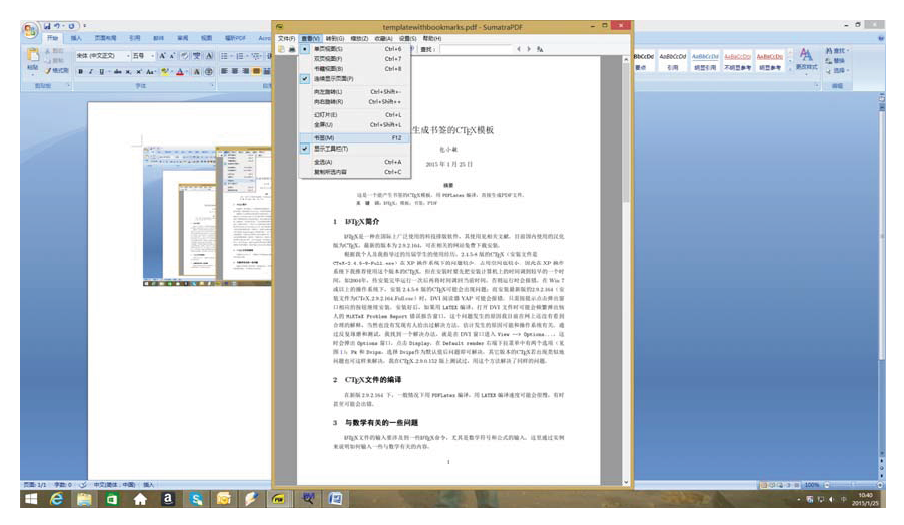
\includegraphics[width=16cm]{codes/selectbookmarks.eps}\\
  \caption{书签的选择}\label{fig:bookmarkselection}
\end{figure}
%---------------------------------------
\subsection{索引的生成\index{索引的生成}}
%---------------------------------------
学院对本科生的毕业论文并没有要求索引,但如果有人想给出索引,那么可以按下面步骤来生成索引:
\begin{enumerate}
  \item 对文章中需要列入索引的词组(如索引)的后面输入\verb=\index{索引}=;
  \item 在主文件中将\%\verb=\makeindex= 前的\%去掉;
  \item 在主文件{ \tt myTemplate.tex} 的编辑窗口上端点击{ \tt TeX},在下拉菜单中点击{\tt Make~Index}(见图~\ref{fig:gensuoyin}),然后再点击{ \tt PDFLaTeX} 编译即可。
\end{enumerate}
\begin{figure}
  \centering
  % Requires \usepackage{graphicx}
  \includegraphics[width=8cm]{gensuoyin.jpg}\\
  \caption{生成索引的操作}\label{fig:gensuoyin}
\end{figure}

%---------------------------------------
\subsection{\CTeX{} 文件编译后产生的附属文件}
%---------------------------------------
%\begin{figure}
%  \centering
%  % Requires \usepackage{graphicx}
%  \includegraphics[width=2cm]{garbagecan.png}\\
%  %\caption{}\label{}
%\end{figure}
\CTeX{} 文件的编译会产生一些附属的文件,如后缀为{\tt .aux,.idx,.log,.out}的文件。在最后的PDF文件编译完成后,如果想删除这些文件,可以点击{\rm WinEdt}窗口上部~GUI 中的\includegraphics[width=.4cm]{garbagecan.png},在弹出的窗口中点击``OK"(见图~\ref{fig:deletewin})即可将相应的文件删除。
\begin{figure}
  \centering
  % Requires \usepackage{graphicx}
  \includegraphics[width=8cm]{deletewin.png}\\
  \caption{删除附属文件的窗口}\label{fig:deletewin}
\end{figure}

%---------------------------------------
\section{与数学有关的一些内容}\label{sec:2two}
%---------------------------------------
\subsection{常见的数学环境\index{数学环境}示例\index{数学环境}}
\LaTeX 文件的输入要涉及到一些 \LaTeX 命令,尤其是数学符号和公式的输入。这里通过实例来说明如何输入一些与数学有关的内容。建议学生在使用前阅读一遍。通过对比PDF文件中的效果和源文件对应的排版命令,初学者可以快速上手使用\LaTeX 。
\begin{definition}
设
\begin{equation}\label{eq:1}
    a_1,a_2,\cdots, a_n, \cdots
\end{equation}
是一个数列。和
$$\sum_{i=1}^n a_i$$
称为数列~\eqref{eq:1} 的前$n$项和。
\end{definition}
\begin{lemma}[新定理]
若$p$是一个素数,且$p$不能够被$a\in \mathbb{N}$整除,则
$$a^{p-1}\equiv 1\pmod{p}.$$
\end{lemma}
\begin{proof}
引理的证明在此给出。
\end{proof}
\begin{theorem}[欧拉定理\index{欧拉定理}]\label{thm:euola}
若$\gcd(a,n) = 1$,则
$$a^{\phi(n)}\equiv 1\pmod{n}.$$
\end{theorem}
\begin{proof}
下面我们来证明这个定理。
\end{proof}
\begin{lemma}[费尔马小定理\index{费尔马小定理}]
若$p$是一个素数\index{素数},且$p$不能够被$a\in \mathbb{N}$整除,则
$$a^{p-1}\equiv 1\pmod{p}.$$
\end{lemma}
\begin{proof}
引理的证明在此给出。
\end{proof}
\begin{corollary} 由组合数的定义立得
$$\binom{n}{k}=\binom{n}{n-k}.$$
\end{corollary}
\begin{property}
性质的内容。
\end{property}
\begin{example}[2011\ 江苏卷]在平面直角坐标系$xOy$中,$M$,$N$分别是椭圆$C$:
$\frac{x^{2}}{4^{2}}+\frac{y^{2}}{2^{2}}=1$的顶点,
过坐标原点的直线交椭圆于$P$,$A$两点,其中点$P$在第一象限.过$P$ 作$x$轴的垂线,
垂足为$C$.连接$AC$,并延长交椭圆与点$B$.设直线$PA$的斜率为$k$.\\
\parbox{10cm}{
\begin{enumerate}
  \item 若直线$PA$平分线段$MN$,求$k$的值;
  \item 当$k=2$时,求点$P$到直线$AB$的距离$d$;
  \item 对任意的$k>0$,求证:$PA\perp PB$.
\end{enumerate}}
%\parbox{3cm}{
%\begin{center}
%\includegraphics[height=3cm,angle=0]{wangyang2}\\
%\caption{椭圆}\label{fig:1}
%\end{center}}
\end{example}

\begin{example}[2010,重庆卷]
例题的内容$\langle ID,\mu,\gamma\rangle$,$\langle ID,\mu,\gamma\rangle$。
\end{example}
\begin{solution}
解答的内容。
\end{solution}
\begin{exercise}
练习题的内容。
\end{exercise}
\begin{note}
注释的内容。
\end{note}
\begin{proposition}
命题的内容。
\end{proposition}
\begin{proof}
命题的证明。
\end{proof}

\subsection{算法的排版\index{}}
用\CTeX 可以排出版面非常漂亮的算法\index{算法的排版}。根据所用宏包的不同,所用的命令也有所不同。下面是用宏包~{\tt algorithm} 和~{\tt algorithmic} 进行算法排版的一个例子。所排的算法是著名的\index{欧几里得算法}欧几里得算法\citeu{stinson}。

%%%%%%%%%%%%%%%%%%%%%%%%%%%%%%%%%%%%%%%%%%%%%%%
\begin{algorithm}
\caption{Euclidean algorithm$(a,b)$}
\label{alg:euclid}
\algsetup{indent=2em}
\begin{algorithmic}[1]
\REQUIRE 整数$a,b\ne 0$
\ENSURE  商序列$q_1,q_2,\cdots,q_m$和$\gcd(a,b)$
\STATE $r_0 \leftarrow a$
\STATE $r_1 \leftarrow b$
\STATE $m\leftarrow 1$
\WHILE{$r_m\ne 0$}
\STATE $q_m\leftarrow\lfloor\frac{r_{m-1}}{r_m}\rfloor$
\STATE $r_m\leftarrow r_{m-1}-q_mr_m$
\STATE $m\leftarrow m+1$
\ENDWHILE
\STATE $m\leftarrow m-1$
\RETURN {$(q_1,q_2,\cdots, q_m;r_m)$}
\STATE {\bf{comment:}$r_m = \gcd(a,b)$ }
\end{algorithmic}
\end{algorithm}
算法~\ref{alg:euclid_no}是另一个标号\index{算法标号}的。
\begin{algorithm}
\caption{Euclidean algorithm$(a,b)$}
\label{alg:euclid_no}
\algsetup{indent=2em}
\begin{algorithmic}[2]
\REQUIRE 整数$a,b\ne 0$
\ENSURE  商序列$q_1,q_2,\cdots,q_m$和$\gcd(a,b)$
\STATE $r_0 \leftarrow a$
\STATE $r_1 \leftarrow b$
\STATE $m\leftarrow 1$
\WHILE{$r_m\ne 0$}
\STATE $q_m\leftarrow\lfloor\frac{r_{m-1}}{r_m}\rfloor$
\STATE $r_m\leftarrow r_{m-1}-q_mr_m$
\STATE $m\leftarrow m+1$
\ENDWHILE
\STATE $m\leftarrow m-1$
\RETURN {$(q_1,q_2,\cdots, q_m;r_m)$}
%\STATE {\bf{comment:}$r_m = \gcd(a,b)$ }
\end{algorithmic}
\end{algorithm}

%\setcounter{algorithm}{4}
下面的算法~\ref{alg:rgg}是一个生成$q$进制$n$元反射Gray码\index{反射Gray码}的算法。
\begin{algorithm}
\caption{\sc Reflected Gray Code Generation$(q, n)$}
\label{alg:genGraycode}
\algsetup{indent=2em}
\begin{algorithmic}
%%\TitleOfAlgo{Euclidean algorithm$(a,b)$}
\label{alg:rgg}
\REQUIRE{整数$q>0,n > 0$}
\ENSURE {$q^n\times n$矩阵$G$}
\STATE $g_{n-1}g_{n-2}\cdots g_{0}\longleftarrow 00\cdots 0$
\WHILE{$(2\mid q$ \AND $g_{n-1},g_{n-2},\cdots ,g_{0} \neq q-1,\bm{0}_{n-1})$ \OR $(2\nmid q$ \AND $g_{n-1},\cdots ,g_{n} \neq \bm{(q-1)}_{n}$}
    \STATE $i\leftarrow 0$
    \STATE $\sigma \leftarrow (g_{n-1}+g_{n-2}+\cdots +g_{i+1})\bmod 2$
    \IF{$\sigma=0$ \AND $g_{i}\neq q-1$}
        \STATE $g_{i} \leftarrow g_{i}+1$
    \ELSIF{$\sigma =1$ \AND $g_{i}\neq 0$}
        \STATE $g_{i}\leftarrow g_{i}-1$
    \ENDIF
    \STATE $i \leftarrow i+1$
    \IF{$i = q-1$}
        \STATE $g_{i} \leftarrow g_{i}+1$
    \ENDIF
\ENDWHILE
\end{algorithmic}
\end{algorithm}
%再来一个不标号不连线的:
%\LinesNotNumbered
%\SetAlgoNoLine
%
%\begin{procedure}[H]
%\caption{$f$()\hspace{-.15cm}$(x,a,b)$}
%\label{proc:f}
%\KwIn{$x,a,b$}
%\uIf{$x\in S_1$}{
%    $f\leftarrow (\beta x,a,(b+1)\bmod n)$
%    }
%\uElseIf{$x\in S_2$}{
%    $f\leftarrow (x^2,2a\bmod n,2b\bmod n)$
%    }
%\Else{
%    $f\leftarrow (\alpha x,(a+1)\bmod n,b)$
%    }
%\Return{$(f)$}
%\end{procedure}
\begin{algorithm}
%\COMMENT{external}% {\bf  External: }}
%\begin{algorithmic}
\caption{{\sc Collision-To-Second-Preimage}\,$(h)$}
\label{algo:c2sec}
\begin{algorithmic}
%\REQUIRE{Hash 函数$h$}
\STATE \bf{External: }{\sc Oracle-2nd-Preimage}
\STATE Choose $x\in_R\mathcal{X}$
\IF{{\sc Oracle-2nd-Preimage}\,$(h,x) = x'$}
    \RETURN $(x,x')$
\ELSE{\RETURN{{\rm(``failure")}}}
\ENDIF
\end{algorithmic}
\end{algorithm}
%---------------------------------------
\section{多栏排版\index{多栏排版}}
%---------------------------------------
多栏环境是一个常用的环境,下面是一个两栏排版的例子。
\begin{Parallel}[v]{0.38\textwidth}{}
\ParallelLText{在最早的
中国求圆学者
中,必须首先
要提到的是张
衡。他是汉朝
的一位著名科
学家。}
\ParallelRText{Among the earliest
Chinese circle-squarers
mention must be made
of Chang Heng in the
first p1ace. He was a famous
scholar of the Han
Dynasty.}
\end{Parallel}
%---------------------------------------
\section{表格、公式与插图\index{插图}}\label{sec:ssss}
%---------------------------------------
\subsection{表格}
%---------------------------------------

%$$\sum_{i=1}^m(-1)^i\binom{m+n-i}{i,m-i,n-i} = \sum_{i=1}^m(-1)^i\binom{m}{i}\binom{m+n-i}{m}, \mbox{其中$m\leq n$}$$


表题应写在表格\index{表格}上方正中,表序写在表题左方不加标点,空一格写表题,表题末尾不加标点,全文的表格统一编序,表序必须连续。
\begin{table}[h]
  \centering
  \caption{一些数学符号的{\LaTeX}输入命令与效果对照表}\label{table:1}
  \begin{tabular}{|c|c|}\hline
  输入 & 输出 \\\hline
  \verb=$(\sum x_{ij})^{1/p}$= & $(\sum x_{ij})^{1/p}$ \\\hline
  \verb=$\left(\sum x_{ij}\right)^{1/p}$= & $\left(\sum x_{ij}\right)^{1/p}$ \\\hline
  \verb=$\bigl(\sum x_{ij}\bigr)^{1/p}$= & $\bigl(\sum x_{ij}\bigr)^{1/p}$ \\\hline
  \verb=$\Bigl(\sum x_{ij}\Bigr)^{1/p}$= & $\Bigl(\sum x_{ij}\Bigr)^{1/p}$ \\\hline
  \verb=$\biggl(\sum x_{ij}\biggr)^{1/p}$= & $\biggl(\sum x_{ij}\biggr)^{1/p}$ \\\hline
  \verb=$\Biggl(\sum x_{ij}\Biggr)^{1/p}$= & $\Biggl(\sum x_{ij}\Biggr)^{1/p}$ \\
  \hline
\end{tabular}
\end{table}
表题用五号宋体居中(见表~\ref{table:1}),表格内中文用五号宋体,英文用五号Times
New Roman字体。

表题允许下页接写,接写时表题省略,表头应重复书写,并在右上方写``续表xx"。下面是一些表格的实例。
%\begin{table}
%\tbl{Radio-band beaming model parameters for\\ {FSRQs and BL Lacs.}}
%{\begin{tabular}[l]{@{}lcccccc}
%\toprule
%  Class$^{\rm a}$ & $\gamma _1$ & $\gamma _2$$^{\rm b}$
%
%         & $\langle \gamma \rangle$
%
%         & $G$ & $|{\bm f}|$ & $\theta _{c}$ \\
%
%\hline%colorrule
%  BL Lacs &5 & 36 & 7 & $-4.0$ & $1.0\times 10^{-2}$ & 10$^\circ$ \\
%  FSRQs & 5 & 40 & 11 & $-2.3$ & $0.5\times 10^{-2}$ & 14$^\circ$ \\
%\bottomrule
%\end{tabular}}
%\tabnote{$^{\rm a}$This footnote shows what footnote symbols to use.}
%\tabnote{$^{\rm b}$This footnote shows the text turning over when a long footnote is added.}
%\label{symbols}
%\end{table}

%\taburulecolor | gray!50|{red} \arrayrulewidth=1pt
%{
%\taburulecolor | yellow |{blue}
%\begin{tabu}{|X|X|} \hline
%Here the lines & are drawn in blue \\ \taburulecolor {green} \hline
%But starting from here & they are green coloured ! \\ \hline
%And now a nested tabu & \begin{tabu}{X} \firsthline\hline
%guess what colour \\ \hline
%is used for rules ?\\ \lasthline \hline
%\end{tabu} \\\hline
%\end{tabu}
%In side the group, rule colors are blue
%}%
%After the group, rule colors are red again !
%\begin{tabu}{X}\hline \hline \indent \end{tabu}


\begin{table}[htb]
 \centering\caption{三线表示例}
\begin{tabular}{ccccc}\toprule
姓名 & 平时成绩 & 期中考试 & 期末考试 & 最后成绩\\\midrule
张三 & 60       & 78       & 76       & 67      \\
李四 & 89       & 92       & 98       & 95      \\
王五 & 95       & 91       & 100      & 97      \\\bottomrule
\end{tabular}
\end{table}
\begin{center}
\begin{tabular}{|c|c|c|c|c|c|c|c|}\hline
\multirow{2}*{题号} & \multicolumn{5}{c|}{第一部分} & \multirow{2}*{第二部分} & \multirow{2}*{总分}\\\cline{2-6}
                    & 一 & 二 & 三 & 四 & 五        &                         & \\\hline
               得分 &    &    &    &    & $\surd$   &                         & \\\hline
\end{tabular}
\end{center}
\begin{table}[htb]
 \centering
 \caption{一班课程表}
   \begin{tabular}{|c| *{7}{c|}}\hline
   \backslashbox{课节}{星期} & 星期一 & 星期二 & 星期三 & 星期四 & 星期五 & 星期六 & 星期日 \\\hline
   1 & & & & & & &  \\\hline
   2 & & & & & & &  \\\hline
   3 & & & & & & &  \\\hline
   4 & & & & & & &  \\\hline
   5 & & & & & & &  \\\hline
   中午& \multicolumn{7}{c|}{}   \\\hline
   6 & & & & & & &  \\\hline
   7 & & & & & & &  \\\hline
   \end{tabular}
\end{table}
%---------------------------------------
\subsection{公式}
%---------------------------------------
公式应另起一行,正文中的公式\index{公式}、算式或方程式等应编排序号,公式的编号用圆括号括起,
序号标注于该式所在行(当有续行时,应标注于最后一行)的行末。公式可按章节顺序编号或按全文统一编号。公式序号必须连续,
不得重复或跳缺。重复引用的公式不得另编新序号。
较长的公式,如必须转行时,最好在等号处转行,如做不到这一点,要在$+,
-, \times, \div$等数学符号处转行。
数学符号应写在转行处的行首。上下式尽可能在等号``="处对齐。
$\sum\limits_{i=1}^nn^2$

\begin{flushleft}
$
\begin{aligned}
  f(x,y) &= f(0,0) + \frac{1}{1!}\left(x\frac{\partial}{\partial x}+y\frac{\partial}{\partial y}\right)f(0,0) \\
         &= \frac{1}{2!}\left(x\frac{\partial}{\partial x}+y\frac{\partial}{\partial y}\right)^2f(0,0) + \cdots\\
         &= \frac{1}{n!}\left(x\frac{\partial}{\partial x}+y\frac{\partial}{\partial y}\right)^nf(0,0) + K
\end{aligned}
$
\end{flushleft}

\[
\begin{aligned}
f(x,y) &= f(0,0) + \frac{1}{1!}\left(x\frac{\partial}{\partial x}+y\frac{\partial}{\partial y}\right)f(0,0) \\
       &= \frac{1}{2!}\left(x\frac{\partial}{\partial x}+y\frac{\partial}{\partial y}\right)^2f(0,0) + \cdots\\
       &= \frac{1}{n!}\left(x\frac{\partial}{\partial x}+y\frac{\partial}{\partial y}\right)^nf(0,0) + K
\end{aligned}
\]
\begin{equation}\label{eq:a}
    \begin{split}
      f(x,y) =& f(0,0) + \frac{1}{1!}\left(x\frac{\partial}{\partial x}+y\frac{\partial}{\partial y}\right)f(0,0) \\
              & + \frac{1}{2!}\left(x\frac{\partial}{\partial x}+y\frac{\partial}{\partial y}\right)^2f(0,0) + \cdots\\
              & + \frac{1}{n!}\left(x\frac{\partial}{\partial x}+y\frac{\partial}{\partial y}\right)^nf(0,0) + K
    \end{split}
\end{equation}
\[ \Set{x\in\mathbf{R} | 0<|x|<\frac{5}{3}} \]
\[
\left\{\vphantom{\frac{5}{3}}x\in\mathbf{R} \right/\left.
0<{|x|}<\frac{5}{3}\right \}
\]
$$S = \sum_{i=1}^n m_i$$
\[\left\{
\begin{aligned}
  a_{11}x + a_{12}y &= b_1 \\
  a_{21}x + a_{22}y &= b_2
\end{aligned}
\right.
\]
方程组只要一个编号
\begin{equation}
\begin{aligned}
  a_{11}x + a_{12}y &= b_1 \\
  a_{21}x + a_{22}y &= b_2\\
  a_{21}x + a_{22}y &= b_2
\end{aligned}
\end{equation}
或者
\begin{equation}
\left\{
\begin{aligned}
  a_{11}x + a_{12}y &= b_1 \\
  a_{21}x + a_{22}y &= b_2
\end{aligned}
\right.
\end{equation}
方程组中如每个方程要单独编号,则可写成
\begin{numcases}{}
%要使用cases package
        a_{11}x + a_{12}y = b_1\label{eq:111} \\
        a_{21}x + a_{22}y = b_2\label{eq:222}
\end{numcases}
\eqref{eq:111}-\eqref{eq:222}
或
\begin{align}
        a_{11}x + a_{12}y &= b_1 \\
        a_{21}x + a_{22}y &= b_2
\end{align}

\[
f(x) =  \left\{
  \begin{array}{ll}
    x+1, & \hbox{if $x>1$;} \\
    -x, & \hbox{if $x\leq 1$.}
  \end{array}
\right.
\]
%---------------------------------------
\makeatother
\subsection{插图}
每幅插图\index{插图}应有图序和图题,全文插图可以统一编序,图序必须连续,不得重复或跳缺。
图序和图题写在图的下方(见图~\ref{fig:1}),五号宋体居中。
\begin{figure}
\centering

\includegraphics[height=6.6cm,angle=0]{preample/ms}\\
\caption{数学与统计学院院徽}\label{fig:1}
\end{figure}
下面是两种图片并列(图~\ref{fig:33} 和图~\ref{fig:44},图~\ref{fig:21}和图~\ref{fig:22})的两种情形:
\begin{figure}[b]
\centering
\begin{minipage}[t]{5cm}
\centering
\mbox{\resizebox{!}{35mm}{
\includegraphics{preample/ms}}}\\
\caption{数学与统计学院院徽}\label{fig:33}
\end{minipage}
\hspace{1.5cm}
\begin{minipage}[t]{5cm}
\centering
 \mbox{\resizebox{!}{15mm}{
\includegraphics{preample/xishi}}}\\
 \caption{西南大学}\label{fig:44}
\end{minipage}
\end{figure}

%%%%%%%%%%%%%%%%%%%%%%%%%%%%%%%%
\begin{figure}
\centering
\mbox{\subfigure[第一个子图]{\resizebox{!}{15mm}{

\includegraphics{preample/xishi}\label{fig:21}
}}}\hspace{1.5cm}
\mbox{\subfigure[第二个子图]{\resizebox{!}{35mm}{

\includegraphics{preample/ms}\label{fig:22}
}}}\\
\caption{西南大学}
\end{figure}
%---------------------------------------
\section{参考文献的引用\index{引用}示例}\label{sec_si4}
%---------------------------------------
按论文中参考文献出现的次序,用中括号的数字连续编号,五号宋体,文献顶格,单倍行距(见例~\ref{li:2})。引用格式按照西南大学学报要求,
请注意标点符号。
国内高等院校数学专业常用的两本\citeu{xiong,zhang}《近世代数》是张禾瑞编著的
《近世代数》\cite{zhang}和熊全淹编著的 《近世代数》\cite{xiong}.
\begin{example}\label{li:2}
参考文献中条目排版示例:
\begin{verbatim}
[4] 郑霖,柴宗新,郑远昌等.四川省地理[M].四川科学技术出版社,
    1994.108-111.
[5] 刘广珠. 高中生考试焦虑成因分析[J].陕西师大学报(哲社版),
    1995,24(1):161-164.
\end{verbatim}
\end{example}
这是一个外文参考文献的引用实例\citeu{experqc}。请注意上面两种引用格式,一种是上标, 一种是正常。使用者可根据自己的喜好选用。

这是另外一种引用方式~\cite{das},如果必要也可以这样用。


\section{程序代码的插入\index{代码的插入}}\label{sec:codeinludsion}如果论文涉及到较长的计算机程序,可以考虑将其放在附录中。使用下面的命令
\begin{verbatim}
        \lstinputlisting[language=代码语言]{代码文件名}
\end{verbatim}
即可将程序代码引入~\CTeX 中,这里``代码语言"是指编写代码所使用的语言,如~{\tt C/C++},{\tt Matlab} 等,而``代码文件名"是指存放代码所使用的文件名(如代码文件存放在与 fulu.txt 不同的文件夹中,
还需给出那个文件夹的路径)。附录~\ref{appendix:A}---\ref{appendix:D}\index{附录}
给出了~{\tt C/C++},{\tt Matlab},{\tt Mathematica} 和~{\tt R} 的具体例子。

